\documentclass[12pt]{report}
\usepackage[margin=1cm]{geometry}
\usepackage[spanish]{babel}
\usepackage[none]{hyphenat}
\usepackage{amsmath} 
\usepackage{parskip} 
\newcommand{\unit}[1]{\ensuremath{\, \mathrm{#1}}}
\usepackage{graphicx}
\usepackage{wrapfig}

\sloppy
\setlength{\parindent}{0cm}
\decimalpoint 
\pagestyle{empty} 

\begin{document}
    \bfseries
    Integración por partes: $\int udv = uv - \int vdu$

    $1) \int x\sen xdx \Rightarrow u = x, dv = \sen xdx \Rightarrow du = dx, v = \int \sen xdx = -\cos x \Longrightarrow \int x\sen xdx = x(-\cos x) - \int (-\cos x)dx = -x\cos x + \int \cos xdx = \boxed{-x\cos x + \sen x + C}$

    $2) \int \ln xdx \Rightarrow u = \ln x, dv = dx \Rightarrow du = \frac{dx}{x}, v = \int dx = x \Longrightarrow \int \ln xdx = \ln x(x) - \int x\frac{dx}{x} = x\ln x - \int dx = x\ln x - x + C = \boxed{x(\ln x - 1) + C}$

    $3) \int x^n\ln xdx \Rightarrow u = \ln x, dv = x^ndx \Rightarrow du = \frac{dx}{x}, v = \int x^ndx = \frac{x^{n+1}}{n+1} \Longrightarrow \int x^n\ln xdx = \ln x \frac{x^{n+1}}{n+1} - \int \frac{x^{n+1}}{n+1}\cdot \frac{dx}{x} = \frac{x^{n+1}}{n+1}\ln x - \frac{1}{n+1}\int \frac {x^{n+1}}{dx} = \frac{x^{n+1}}{n+1}\ln x - \frac{1}{n+1}\cdot \frac{x^{n+1}}{n+1} + C = \boxed{\frac{x^{n+1}}{n+1}(\ln x - \frac{1}{n + 1}) + C}$

    $4) \int xe^{ax}dx \Rightarrow u = x, dv = e^{ax}dx \Rightarrow du = dx, v = \int e^{ax}dx = \frac{e^{ax}}{a} \Longrightarrow \int xe^{ax}dx = x\frac{e^{ax}}{a} - \int \frac{e^{ax}}{a}dx = x\frac{e^{ax}}{a} - \frac{1}{a} \int e^{ax}dx = x\frac{e^{ax}}{a} - \frac{1}{a}\frac{e^{ax}}{a} + C = \boxed{\frac{e^{ax}}{a}(x - \frac{1}{a}) + C}$

    $5) \int \arctan xdx \Rightarrow u = \arctan x, dv = dx \Rightarrow du = \frac{dx}{1+x^2}, v \int dx = x \Longrightarrow \int \arctan xdx = \arctan(x) - \int \frac{dx}{1+x^2}dx = x\arctan x - \int \frac{xdx}{1+x^2} = \boxed{x\arctan x - \frac{1}{2}\ln (1+x^2) + C}$

    $6) \int e^{-2x}\sen e^{-x}dx \Rightarrow u = e^{-x} \Rightarrow du = -e^{-x}dx \Rightarrow dx = -\frac{du}{e^{-x}} = -\frac{du}{u} \Rightarrow dv = e^{-2x}\sen udx \Rightarrow \int e^{-2x}\sen e^{-x}dx = \int e^{-x}\cdot e^{-x}\sen e^{-x} = u\cdot u\sen u(-\frac{du}{u}) = - \int u\sen udu \Longrightarrow I = \int e^{-2x}\sen e^{-x}dx = -(-u\cos u + \sen u + C_1) = \boxed{+e^{-x}\cos e^{-x} - \sen e^{-x} + C} \Rightarrow C = -C_1$

    Integrales resolubles mediante integración por partes \\
    Forma A: $\int x^ne^{ax}dx$, $\int x^n\sen axdx$, o $\int x^n\cos axdx$ hacer $u = x^n$ y $dv = e^{ax}dx, \sen axdx, \cos axdx$ \\
    Forma B: $\int x^n\ln xdx$, $\int x^n\arcsen axdx$, o $\int x^n\arccos axdx$ hacer $u = \ln x, \arcsen ax, \arccos ax$ y $dv = x^ndx$ \\
    Forma C: $\int e^{ax}\sen bxdx$ o $\int e^{ax}\cos bxdx$ hacer $u = e^{ax}$ y $dv = \sen bxdx, \cos bxdx$ \\

    Integración por sustitución trigonométrica \\
    $\sqrt{a^2-u^2} \Rightarrow u = a\sen\theta \Rightarrow du = a\cos\theta d\theta \Rightarrow \sqrt{a^2-u^2} = a\cos\theta$ \\
    $\sqrt{a^2+u^2} \Rightarrow u = a\tan\theta \Rightarrow du = a\sec^2\theta d\theta \Rightarrow \sqrt{a^2+u^2} = a\sec\theta$ \\
    $\sqrt{u^2-a^2} \Rightarrow u = a\sec\theta \Rightarrow du = a\sec\theta \tan\theta d\theta \Rightarrow \sqrt{u^2-a^2} = a\tan\theta$
    
    $1) \int \frac{du}{\sqrt{a^2-u^2}} \Rightarrow u = a\sen\theta \Rightarrow du = a\cos\theta d\theta \Rightarrow \theta = \arcsen\frac{u}{a} \Rightarrow \sqrt{a^2-u^2} = \sqrt{a^2-a^2\sen^2\theta} = \sqrt{a^2(1-\sen^2\theta)} = \sqrt{a^2\cos^2\theta} = a\cos\theta \Longrightarrow I = \int \frac{du}{\sqrt{a^2-u^2}} = \int \frac{a\cos\theta d\theta}{a\cos\theta} = \int d\theta = \theta + C = \arcsen\frac{u}{a} + C \Rightarrow \int \frac{du}{\sqrt{a^2-u^2}} = \boxed{\arcsen\frac{u}{a} + C}$

    $2) \int\frac{du}{u^2+a^2} \Rightarrow u = a\tan\theta \Rightarrow du = a\sec^2\theta d\theta \Rightarrow \theta = \arctan\frac{u}{a} \Rightarrow \sqrt{a^2+u^2} = \sqrt{a^2+a^2\tan^2\theta} = \sqrt{a^2(1+\tan^2\theta)} = \sqrt{a^2\sec^2\theta} = a\sec\theta \Longrightarrow I = \int\frac{du}{u^2+a^2} = \int\frac{du}{(\sqrt{u^2+a^2})^2} = \int\frac{a\sec^2\theta d\theta}{(a\sec\theta)^2} = \int\frac{a\sec^2\theta}{a^2\sec^2\theta}d\theta = \frac{1}{a}\int d\theta = \frac{1}{a}\theta + C = \frac{1}{a}\arctan\frac{u}{a} + C \Rightarrow \int\frac{du}{u^2+a^2} = \boxed{\frac{1}{a}\arctan\frac{u}{a} + C}$

    $3) \int\frac{du}{u\sqrt{u^2-a^2}} \Rightarrow u = a\sec\theta \Rightarrow du = a\sec\theta\tan\theta d\theta \Rightarrow \theta = arcsec\frac{|u|}{a} \Rightarrow \sqrt{u^2+a^2} = \sqrt{a^2\sec^2\theta - a^2} = \sqrt{a^2(\sec^2\theta - 1)} = \sqrt{a^2\tan^2\theta} = a\tan\theta \Longrightarrow I = \int\frac{du}{u\sqrt{u^2-a^2}} = \int\frac{a\sec\theta\tan\theta d\theta}{(a\sec\theta)(a\tan\theta)} = \frac{1}{a}\int d\theta = \frac{1}{a}\theta + C = \frac{1}{a}arcsec\frac{|u|}{a} + C \Rightarrow \int\frac{du}{u\sqrt{u^2-a^2}} = \boxed{\frac{1}{a}arcsec\frac{|u|}{a} + C}$

    $4) \int\sqrt{r^2-x^2}dx \Rightarrow a^2 = r^2 \Rightarrow a = r \Rightarrow u^2 = x^2 \Rightarrow u = x \Rightarrow x = r\sen\theta \Rightarrow dx = r\cos\theta d\theta \Rightarrow \sen\theta = \frac{x}{r} \Rightarrow \sqrt{r^2-x^2} = \sqrt{r^2-(r\sen\theta)^2} = \sqrt{r^2\cos^2\theta} = r\cos\theta \Rightarrow \cos\theta = \frac{\sqrt{r^2-x^2}}{r} \Rightarrow \theta = \arccos \frac{\sqrt{r^2-x^2}}{r}$ o $\theta = \arcsen \frac{x}{r} \Longrightarrow I = \int\sqrt{r^2-x^2}dx = \int r\cos\theta(r\cos\theta d\theta) = r^2\int\cos^2\theta d\theta = \frac{r^2}{2}\int(1+\cos 2\theta)d\theta = \frac{r^2}{2}\int d\theta + \frac{r^2}{2}\int\cos 2\theta d\theta = \frac{r^2}{2}\theta + \frac{r^2}{2}\frac{\sen 2\theta}{2} + C \Rightarrow \sen 2\theta = 2\sen\theta\cos\theta \Longrightarrow I = \frac{r^2}{2}\theta + \frac{r^2}{2}\frac{\sen 2\theta}{2} + C = \frac{r^2}{2}\theta + \frac{r^2}{2}\frac{2\sen\theta\cos\theta}{2} + C = \frac{r^2}{2}\theta + \frac{r^2}{2}\sen\theta\cos\theta + C = \frac{r^2}{2}\arcsen\frac{x}{r} + \frac{r^2}{2}\frac{x}{r}\frac{\sqrt{r^2-x^2}}{r} + C = \boxed{\frac{r^2}{2}\arcsen\frac{x}{r} + \frac{x}{2}\sqrt{r^2-x^2} + C}$

    $5) \int\sqrt{9x^2+1}dx \Rightarrow a = 1 \Rightarrow u = 3x \Rightarrow 3x = 1\cdot\tan\theta \Rightarrow x = \frac{1}{3}\tan\theta \Rightarrow dx = \frac{1}{3}\sec^2\theta d\theta \Rightarrow \sqrt{9x^2 + 1} = 1\cdot\sec\theta \Rightarrow \theta=\arctan 3x \Rightarrow \theta = arcsec \sqrt{9x^2+1} \Longrightarrow I = \int\sqrt{9x^2+1}dx = \int\sec\theta(\frac{1}{3}\sec^2\theta d\theta) = \frac{1}{3}\int\sec^3\theta d\theta = \frac{1}{3}[\frac{1}{2}(\sec\theta\cdot\tan\theta + \ln|\sec\theta + \tan\theta|)] + C = \frac{1}{6}(\sqrt{9x^2+1}\cdot3x + \ln|\sqrt{9x^2+1} + 3x|) + C = \frac{3x\sqrt{9x^2+1}}{6} + \frac{1}{6}\ln|\sqrt{9x^2+1} +3x| + C = \frac{x\sqrt{9x^2+1}}{2} + \frac{1}{6}\ln|\sqrt{9x^2+1} +3x| + C = \boxed{\frac{x\sqrt{9x^2+1}}{2} + \ln|\sqrt{9x^2+1} +3x|^{\frac{1}{6}} + C}$

    $6) \sqrt{x^2 - 4}dx \Rightarrow a = 2 \Rightarrow x = 2\sec\theta \Rightarrow dx = 2\sec\theta \tan\theta d\theta \Rightarrow \sqrt{x^2 - 4}dx = 2\tan\theta \Rightarrow \tan\theta = \frac{\sqrt{x^2 - 4}}{2} \Rightarrow \theta = \arctan \frac{\sqrt{x^2 - 4}}{2}$ o $\theta = arcsec\frac{x}{2} \Longrightarrow I = \int\sqrt{x^2 - 4}dx = \int 2\tan\theta\cdot(2\sec\theta\tan\theta d\theta) = 4\int\tan^2\theta\sec\theta d\theta = 4\int(\sec^2\theta - 1)\sec\theta d\theta = 4\int\sec^3\theta d\theta - 4\int\sec\theta d\theta = 4(\frac{1}{2}(\sec\theta\cdot\tan\theta + \ln|\sec\theta + \tan\theta|)) - 4\ln|\sec\theta + \tan\theta| + C = 2\sec\theta\cdot\tan\theta + 2\ln|\sec\theta + \tan\theta| - 4\ln|\sec\theta + \tan\theta| + C =  2\sec\theta\cdot\tan\theta - 2\ln|\sec\theta + \tan\theta| + C  = 2(\frac{x}{2})(\frac{\sqrt{x^2-4}}{2}) - 2\ln|\frac{x}{2} + \frac{\sqrt{x^2-4}}{2}| + C = \boxed{\frac{x\sqrt{x^2-4}}{2} - 2\ln|\frac{x + \sqrt{x^2-4}}{2}| + C}$
    
    \hfill \break
    Integración por descomposición en fracciones racionales. Factores lineales: $\frac{A}{ax + b}$, $\frac{A}{(ax + b)^n}$ \\
    Caso 1. Los factores del denominador son todos de primer grado y distintos, de la forma $\frac{A}{ax + b}$ \\
    $1) \int\frac{4}{x^2-x}dx \Rightarrow \frac{4}{x^2-x} = \frac{4}{x(x-1)} = \frac{A}{x}+\frac{B}{x-1} \Rightarrow 4 = \frac{(x)(x-1)A}{x} +\frac{(x)(x-1)B}{x-1} \Rightarrow 4 = A(x-1) + Bx = Ax - A + Bx = x(A + B) - A \Rightarrow 
    \begin{bmatrix}
        1 & 1 & 0\\
        -1 & 0 & 4
    \end{bmatrix}
    \Rightarrow -A = 4 \Rightarrow \boxed{A = -4} \Rightarrow A + B = 0 \Rightarrow - 4 + B = 0 \Rightarrow \boxed{B = 4} \Longrightarrow \frac{4}{x^2-x} = \frac{-4}{x} + \frac{4}{x-1} \Longrightarrow I = \int\frac{4}{x^2-x}dx = \int\frac{-4}{x} + \int\frac{4}{x-1}dx = -4\ln x + 4\ln(x-1) + C = 4[\ln(x-1) - \ln x] + C = \boxed{\ln(\frac{x-1}{x})^4 + C}$ 

    $2) \int\frac{dx}{4x^3-x} \Rightarrow \frac{1}{4x^3-x} = \frac{1}{x(4x^2-1)} = \frac{1}{x(2x+1)(2x-1)} = \frac{A}{x} + \frac{B}{2x+1} + \frac{C}{2x-1} \Rightarrow 1 = A(2x+1)(2x-1) + Bx(2x-1) + Cx(2x+1) = A(4x^2-1) + B(2x^2-x) + C(2x^2+x) \Rightarrow 1 = x^2(4A + 2B + 2C) + x(-B + C) - A \Rightarrow 
    \begin{bmatrix}
        -1 & 0 & 0 & 1 \\
        0 & -1 & 1 & 0 \\
        4 & 2 & 2 & 0 \\
    \end{bmatrix} \sim 4R_1 + R_3\sim 
    \begin{bmatrix}
        -1 & 0 & 0 & 1 \\
        0 & -1 & 1 & 0 \\
        0 & 2 & 2 & 4 \\
    \end{bmatrix} \sim \frac{1}{2}R_3\sim 
    \begin{bmatrix}
        -1 & 0 & 0 & 1 \\
        0 & -1 & 1 & 0 \\
        0 & 1 & 1 & 2 \\
    \end{bmatrix} \sim R_3 + R_2\sim 
    \begin{bmatrix}
        -1 & 0 & 0 & 1 \\
        0 & 0 & 2 & 2 \\
        0 & 1 & 1 & 2 \\
    \end{bmatrix}
    \Rightarrow 2C = 2 \Rightarrow \boxed{C = 1} \Rightarrow B + C = 2 \Rightarrow B + 1 = 2 \Rightarrow \boxed{B = 1} \Rightarrow -A = 1 \Rightarrow \boxed{A = -1} \Longrightarrow \int\frac{-1}{x}dx + \int\frac{1}{2x+1}dx + \int\frac{1}{2x-1}dx = -\ln x + \frac{1}{2}\ln(2x+1) + \frac{1}{2}\ln(2x-1) + C = \boxed{\ln\frac{\sqrt{(4x^2-1)}}{x} + C}$

    Caso 2. Los factores del denominador son todos de primer grado y algunos es repiten, correspondiéndole la forma $\frac{A}{(ax + b)^n} + \frac{B}{(ax+b)^{n-1}} +...+ \frac{L}{(ax+b)}$
    
    $3) \int\frac{x+5}{x^3-3x+2}dx \Rightarrow x^3-3x+2 = (x+2)(x-1)^2 \Rightarrow \frac{x+5}{3x^2-3x+2} = \frac{x+5}{(x+2)(x-1)^2} = \frac{A}{x+2} + \frac{B}{(x-1)^2} + \frac{C}{x-1} \Rightarrow x + 5 = A(x-1)^2 + B(x+2) + C(x+2)(x-1) = A(x^2-2x+1) + B(x+2) + C(x^2+x-2) = x^2(A + C) + x(-2A + B + C) + (A + 2B - 2C) \Rightarrow
    \begin{bmatrix}
        1 & 0 & 1 & 0 \\
        -2 & 1 & 1 & 1 \\
        1 & 2 & -2 & 5 \\
    \end{bmatrix} \sim 2R_1 + R_2, -1R_1 + R_3\sim 
    \begin{bmatrix}
        1 & 0 & 1 & 0 \\
        0 & 1 & 3 & 1 \\
        0 & 2 & -3 & 5 \\
    \end{bmatrix} \sim -2R_2 + R_3\sim 
    \begin{bmatrix}
        1 & 0 & 1 & 0 \\
        0 & 1 & 3 & 1 \\
        0 & 0 & -9 & 3 \\
    \end{bmatrix}
    \Rightarrow -9C = 3 \Rightarrow C = -3/9 \Rightarrow \boxed{C = -1/3} \Rightarrow B + 3C = 1 \Rightarrow B - 1 = 1 \Rightarrow \boxed{B = 2} \Rightarrow A + C  = 0 \Rightarrow A = -C \Rightarrow \boxed{A = 1/3} \Longrightarrow I = \int\frac{x+5}{x^3-3x+2}dx =\int\frac{1/3}{x+2}dx + \int\frac{2}{(x-1)^2}dx + \int\frac{-1/3}{x-1}dx = \frac{1}{3}\ln|x+2| - \frac{2}{x-1} - \frac{1}{3}\ln|x-1| + C = \frac{1}{3}\ln\frac{x+2}{x-1}-\frac{2}{x-1} + C = \boxed{\ln|\frac{x+2}{x-1}|^{\frac{1}{3}} - \frac{2}{x-1} + C}$

    $4) \int\frac{x^4-2x^2+4x+1}{x^3-x^2-x+1}dx \Rightarrow \frac{x^4-2x^2+4x+1}{x^3-x^2-x+1} = x + 1 + \frac{4x}{x^3-x^2-x+1} \Rightarrow x^3-x^2-x+1 = x^2(x+1) - 1(x-1) = (x-1)(x^2-1) = (x-1)(x-1)(x+1) = (x-1)^2(x+1) \Rightarrow \frac{4x}{x^3-x^2-x+1} = \frac{4x}{(x-1)^2(x+1)} = \frac{A}{(x-1)^2} + \frac{B}{x-1} + \frac{C}{x+1} \Rightarrow 4x = A(x+1) + B(x-1)(x+1) + C(x-1)^2 = A(x+1) + B(x^2-1) + C(x^2-2x+1) = x^2(B + C) + x(A - 2C) + (A- B + C)
    \begin{bmatrix}
        0 & 1 & 1 & 0 \\
        1 & 0 & -2 & 4 \\
        1 & -1 & 1 & 0 \\
    \end{bmatrix} \sim -1R_2 + R_3\sim 
    \begin{bmatrix}
        0 & 1 & 1 & 0 \\
        1 & 0 & -2 & 4 \\
        0 & -1 & 3 & -4 \\
    \end{bmatrix} \sim 1R_1 + R_3\sim 
    \begin{bmatrix}
        0 & 1 & 1 & 0 \\
        1 & 0 & -2 & 4 \\
        0 & 0 & 4 & -4 \\
    \end{bmatrix}
    \Rightarrow 4C = -4 \Rightarrow \boxed{C = -1} \Rightarrow A - 2C = 4 \Rightarrow A = 4 - 2 \Rightarrow \boxed{A = 2} \Rightarrow B + C = 0 \Rightarrow \boxed{B = 1} \Longrightarrow I = \int\frac{x^4-2x^2+4x+1}{x^3-x^2-x+1}dx = \int[x + 1 + \frac{2}{(x-1)^2} + \frac{1}{x-1} + \frac{-1}{x+1}]dx = \frac{x^2}{2} + x - \frac{2}{x-1} + \ln|x-1| - \ln|x+1| + C = \boxed{\frac{x^2}{2} + x - \frac{2}{x-1} + \ln\frac{|x-1|}{|x+1|} + C}$

    \hfill \break
    Área entre dos curvas que se intersectan en dos puntos \\
    Encontrar el área limitada por la hipérbola $xy = 4$ y la recta $x+y=5$. \\
    $f(x) = y = 5 - x \Rightarrow g(x) = y = \frac{4}{x}$ \\
    Puntos de intersección: $f(x) = g(x) \Rightarrow 5-x = 4/x \Rightarrow 5x -x^2 = 4 \Rightarrow x^2-5x+4 = 0 \Rightarrow (x-4)(x-1) = 0$ \\
    $\Rightarrow \underline{(x-1) = 0} \Rightarrow x_1 = 1 \Rightarrow y = 5 - (1) \Rightarrow (1, 4) \Longrightarrow \underline{(x-4) = 0}  \Rightarrow x_2 = 4 \Rightarrow y = 5 - (4) \Rightarrow (4, 1) \Longrightarrow \boxed{[1, 4]}$ \\
    Para saber que función esta arriba o abajo: para $x = 2$\\
    $f(x) = y = \underline{5-x} \Rightarrow f(2) = 5 - 2 = 3 \Longrightarrow g(x) = y = \underline{\frac{4}{x}} \Rightarrow g(2) = \frac{4}{2} = 2 \Longrightarrow \boxed{f(x) $ esta arriba y $ g(x) $ esta debajo: $ g(x) \leq f(x)}$ \\
    Por lo tanto, el área entre las funciones f y g en el intervalo, es: $A = \int_{1}^{4}[f(x)-g(x)]\,dx \int_{1}^{4}[(5-x)-(\frac{4}{x})]\,dx = 5\int_{1}^{4}\,dx - \int_{1}^{4}x\,dx - 4\int_{1}^{4}\frac{dx}{x} = [5x - \frac{x^2}{2} - 4\ln|x|]_{1}^{4} = (5(4) - \frac{4^2}{2} - 4\ln|4|) - (5(1) - \frac{1^2}{2} - 4\ln|1|) = 20 - 8 - 4\ln|4| - 5 + \frac{1}{2} + 0 = 7 + \frac{1}{2} - 4\ln|4| = \frac{15}{2} - 4\ln|4| = 7.5 - 4\ln|4| = \boxed{1.954822556 \unit{u^2}}$

    \hfill \break
    Área entre dos curvas que se intersectan en más de dos puntos \\
    Encontrar el área de la región comprendida entre las gráficas de $f(x) = x^3 + 2$ y $g(x) = x+2$. \\
    Puntos de intersección: $f(x) = g(x) \Rightarrow x^3+2 = x+2 \Rightarrow x^3+2-x-2 = 0 \Rightarrow x^3-x = 0 \Rightarrow x(x^2-1) = 0 \Rightarrow \underline{x = 0} \Rightarrow \boxed{x_1 = 0} \Rightarrow x^2-1 = 0 = (x-1)(x+1) = 0 \Rightarrow \underline{x+1 = 0} \Rightarrow \boxed{x_2 = -1} \Rightarrow \underline{x-1 = 0} \Rightarrow \boxed{x_3 = 1}$ \\
    Las gráficas se cortan cuando $x = 1, 0, -1$: Si $g(x) = x+2$ \\
    $\Rightarrow x = -1 \Rightarrow g(-1) = -1+2 = 1 \Rightarrow (-1, 1)$\\
    $\Rightarrow x = 0 \Rightarrow g(0) = 0+2 = 2 \Rightarrow (0, 2)$\\
    $\Rightarrow x = 1 \Rightarrow g(1) = 1+2 = 3 \Rightarrow (1, 3)$\\
    Los intervalos van en el orden: $(-1, 1), (0, 2), (1, 3) \Rightarrow $ intervalos $\boxed{[-1, 0], [0, 1]}$ \\
    Para saber que función esta arriba o abajo: a) para los puntos $(-1, 1)$ y $(0, 2)$, es decir, el intervalo $[-1, 0]$, entonces $x = -1/2$ (la mitad)\\
    $f(x) = x^3+2 \Rightarrow f(-\frac{1}{2}) = (-\frac{1}{2})^3+2 = -\frac{1}{8} + 2 = \frac{-1+16}{8} = \frac{15}{8} \Longrightarrow g(x) = x+2  \Rightarrow g(-\frac{1}{2}) = -\frac{1}{2}+2 = -\frac{3}{2} \Longrightarrow \boxed{f(x)$ esta arriba y $g(x)$ esta debajo: $\frac{3}{2}\leq\frac{15}{8} \Rightarrow g(x)\leq f(x)}$
    b) para los puntos $(0, 2)$ y $(1, 3)$, es decir, el intervalo $[0, 1]$, entonces $x = 1/2$ (la mitad)\\
    $f(x) = x^3+2 \Rightarrow f(\frac{1}{2}) = (\frac{1}{2})^3+2 = \frac{1}{8} + 2 = \frac{1+16}{8} = \frac{17}{8} \Longrightarrow g(x) = x+2  \Rightarrow g(\frac{1}{2}) = \frac{1}{2}+2 = -\frac{5}{2} \Longrightarrow \boxed{g(x)$ esta arriba y $f(x)$ esta debajo: $\frac{17}{8}\leq\frac{5}{2} \Rightarrow f(x)\leq g(x)}$\\
    Entonces se necesitan dos integrales, una para el intervalo $[-1, 0]$ y otra para el intervalo $[0, 1]$: $A = \int_{-1}^0[f(x)-g(x)]dx + \int_0^1[g(x)-f(x)]dx = \int_{-1}^0[(x^3+2) - (x+2)]dx + \int_0^1[(x+2)-(x^3+2)]dx = \int_{-1}^0(x^3-x)dx + \int_0^1(-x^3+x)dx = [\frac{x^4}{4} - \frac{x^2}{2}]_{-1}^0 + [-\frac{x^4}{4} + \frac{x^2}{2}]_0^1 = 0 - [\frac{(-1)^4}{4} - \frac{(-1)^2}{2}] + [-\frac{1^4}{4} + \frac{1^2}{2}] - 0 = -[\frac{1}{4} - \frac{1}{2}] + [-\frac{1}{4} + \frac{1}{2}] = \frac{1}{4} + \frac{1}{4} = \boxed{\frac{1}{2} \unit{u^2}}$ 

    \hfill \break
    Volumen de un sólido de revolución: Método de discos\\
    Eje de revolución OX, $y = f(x), [a,b] \Longrightarrow V = \pi\int_a^b[f(x)]^2dx$ \\
    Eje de revolución OY, $x = g(y), [c,d] \Longrightarrow V = \pi\int_c^d[g(y)]^2dy$

    1) Encontrar el volumen que se obtiene al hacer girar la región limitada por las curvas con ecuaciones $y = f(x) = \sqrt{x-1} = 0$ y $x = 2$, alrededor del eje de las abscisas (OX), es: $y = \sqrt{x-1} = 0 \Rightarrow x = 1 \Rightarrow \boxed{[1, 2]}$ \\
    Si $x-1 \geq 0 \Rightarrow x \geq 1$, si $x = 1 \Rightarrow y = 0$ \\
    $V = \pi\int_a^b[f(x)]^2dx = \pi\int_1^2[(x-1)^{\frac{1}{2}}]^2dx = \pi\int_1^2(x-1)dx = \pi(\frac{x^2}{2}-x)]_1^2 = \pi[(\frac{2^2}{2}-2) - (\frac{1^2}{2}-1)] = \pi[0 + \frac{1}{2}] = \boxed{\frac{\pi}{2} \unit{u^3}}$

    2) Encontrar el volumen del sólido formado al girar la región acotada por las gráficas de $y = x^2+1$, $x= 0$ y $y = 2$ alrededor del eje OY, como se muestra en la figura: $y = x^2+1 \Rightarrow x = \sqrt{y-1} \Rightarrow y-1 \geq 0 \Rightarrow y \geq 1 \Rightarrow$ si $y = 1 \Rightarrow x = 0 \Rightarrow [c, d] =\boxed{[1, 2]}$ \\
    $V = \pi\int_c^d[g(y)]^2dy = V = \pi\int_1^2[(y-1)^{\frac{1}{2}}]^2dy = \pi\int_1^2(y-1)dy = \pi(\frac{y^2}{2}-y)]_1^2 = \pi[(\frac{2^2}{2}-2) - (\frac{1^2}{2}-1)] = \pi[0 - (-\frac{1}{2})] = \boxed{\frac{\pi}{2} \unit{u^3}}$

    \hfill \break 
    Volumen de un sólido de revolución: Método de las arandelas o del anillo \\ 
    Radio exterior $R(x)$ y radio interior $r(x)$: $V = \pi\int_a^b[[R(x)]^2-[r(x)]^2]dx$ \\  
    Radio exterior $R(y)$ y radio interior $r(y)$: $V = \pi\int_c^d[[R(y)]^2-[r(y)]^2]dy$ 

    3) Encontrar el volumen del sólido formado al girar la región acotada para las gráficas de $y = \sqrt{x}$ y $y = x^2$, alrededor del eje OX. \\
    Para encontrar los puntos de intersección de las gráficas: $x^2 = \sqrt{x} \Rightarrow x^2 - x^{\frac{1}{2}} = 0 \Rightarrow x^{\frac{1}{2}}(x^{\frac{3}{2}}-1) = 0 \Rightarrow x^{\frac{1}{2}}(x^{\frac{3}{4}} + 1)(x^{\frac{3}{4}} - 1) = 0 \Rightarrow \underline{x^{\frac{1}{2}} = 0} \Rightarrow x_1 = 0 \Rightarrow \underline{x^{\frac{3}{4}} + 1 = 0} \Rightarrow x_2 =$ imaginario $\underline{x^{\frac{3}{4}} - 1 = 0} \Rightarrow x_3 = 1$ \\
    Para $y = f(x) = x^2 \Longrightarrow f(0) = 0^2 = 0 \Rightarrow \boxed{(0,0)} \Longrightarrow f(1) = 1^2 = 1 \Rightarrow \boxed{(1,1)}$ \\
    Aplicando la ecuación (1), se tiene que integrando entre $a = 0$ y $b = 1$, se tiene: $V = \pi\int_a^b[[R(x)]^2-[r(x)]^2]dx = \pi\int_0^1[[\sqrt{x}]^2-[x^2]^2]dx = \pi\int_0^1(x-x^4)dx = \pi[\frac{x^2}{2} - \frac{x^5}{5}]_0^1 = \pi[(\frac{1^2}{2} - \frac{1^5}{5}) - 0] = \pi(\frac{1}{2} - \frac{1}{5}) = \pi(\frac{5-2}{10}) = \pi(\frac{3}{10}) = \boxed{\frac{3\pi}{10} \unit{u^3}}$
    
    4) Encontrar el volumen del sólido formado al girar la región acotada por las gráficas de $y = x^2+1$, $y = 0$, $x = 0$ y $x = 1$, alrededor del eje OY, como se muestra en la figura: 
    \begin{wrapfigure}{r}{0.4\textwidth}
        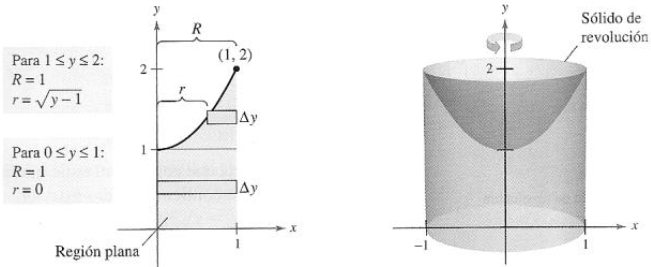
\includegraphics[width=0.4\textwidth]{Solidos1.png}
    \end{wrapfigure}
    Los radios exterior e interior son: \\
    Para $0 \leq y\geq 1 \\\Rightarrow R(y) = 1, r(y) = 0$ \\
    Para $1 \leq y\geq 2 \\\Rightarrow R(y) = 1, r(y) = \sqrt{y-1}$ \\

    Se tiene: \\
    $a = 0$, $b = 1$ y $c = 1$, $d = 2$ \\ 
    $V = \pi\int_0^1[[R(y)]^2-[r(y)]^2]dy + \pi\int_1^2[[R(y)]^2-[r(y)]^2]dy =  \pi\int_0^1([1]^2-[0]^2)dy + \pi\int_1^2([1]^2-[\sqrt{y-1}]^2)dy = \pi\int_0^1(1-0)dy + \pi\int_1^2(1-(y-1))dy = \pi\int_0^1dy + \pi\int_1^2(2-y)dy = \pi[y]_0^1 + \pi[2y - \frac{y^2}{2}]_1^2 = \pi[1-0] + \pi[(2(2) - \frac{2^2}{2}) - (2(1) - \frac{1^2}{2})] = \pi + \pi[2 - \frac{3}{2}] = \pi + \frac{\pi}{2} = \boxed{\frac{3\pi}{2} \unit{u^3}}$

    \hfill \break
    Volumen de un sólido de revolución: Método de las capas \\
    Eje de revolución horizontal: $V = 2\pi\int_c^d yg(y)dy$ \\
    Eje de revolución vertical: $V = 2\pi\int_c^d xf(x)dx$ 

    5) Encontrar el volumen del sólido formado al girar la región acotada por las gráficas de $y = x^2+1$, $y = 0$, $x = 0$ y $x = 1$, alrededor del eje OY: Si $y = x^2+1 \Longrightarrow \underline{x = 0} \Rightarrow y = 1 \Rightarrow (0, 1) \Longrightarrow \underline{x = 1} \Rightarrow y = 2 \Rightarrow (1, 2)$\\
    $V = 2\pi\int_a^b xf(x)dx = 2\pi\int_0^1 x(x^2+1)dx = 2\pi\int_0^1 (x^3+x)dx = 2\pi[\frac{x^4}{4}+\frac{x^2}{2}]_0^1 = 2\pi[(\frac{1^4}{4}+\frac{1^2}{2}) - 0] = 2\pi[\frac{1}{4}+\frac{1}{2}] = \frac{2\pi\cdot3}{4} = \boxed{\frac{3\pi}{2} \unit{u^3}}$
\end{document}